\section{Družina \texorpdfstring{\(\lambda e^z\)}{\lambda exp(z)}}

Dokazali smo, da je \(e^z\) kaotična na celi kompleksni ravnini. Za splošno kompleksno preslikavo pa to ne drži. V tem poglavju bomo preučili dinamiko \emph{eksponentne družine}
\[E_\lambda (z) \coloneq \lambda e^z.\]
Pokažemo, da za \(0 < \lambda < 1/e\), Juliajeva množica \(J (E_\lambda)\) \emph{Cantorjev šopek}. Razdelek je povzet po~\cite[razdelek 9]{Pineiro_2025}.

\subsection{Periodične točke}

Začnemo s preučevanjem realnih fiksnih točk za \(\lambda \in \RR\).

\begin{trditev}
    Naj bo \(\lambda \in \RR\). Potem o realnih fiksnih točkah eksponentne družine lahko povemo naslednje.
    \begin{enumerate}[label=(\arabic*)]
        \item Če je \(\lambda = 1/e\), ima \(E_\lambda\) eno realno fiksno točko \(x^* = 1\).
        \item Če je \(\lambda > 1/e\), potem \(E_\lambda\) nima realnih fiksnih točk.
        \item Če je \(0 < \lambda < 1/e\), potem ima \(E_\lambda\) dve realni fiksni točki: \(x^* \in (0, 1)\) (privlačna) ter \(x^{**} > 1\) (odbojna).
        \item Če je \(\lambda < 0\), potem ima \(E_\lambda\) eno realno fiksno točko \(x^*\):
            \begin{itemize}
                \item \(x^*\) je privlačna za \(-e < \lambda < 0\);
                \item \(x^*\) je odbojna za \(\lambda < -e\);
                \item \(x^*\) je nevtralna za \(\lambda = 1\).
            \end{itemize}
    \end{enumerate}
\end{trditev}

\begin{dokaz}
    (1) Naj bo \(\lambda = 1/e\). Potem je \(E_\lambda (1) = e/e = 1\). Ker je \(E_\lambda' (x^*) = \lambda e^{x^*} = x^* = 1\), je to nevtralna fiksna točka. Ker je premica \(y = ex\) tangenta na \(y = e^x\) v točki \(x = 1\), drugih fiksnih točk ni.

    (2) Naj bo \(\lambda > 1/e\). Pokažemo, da je \(f (x) = \lambda e^x - x > 0\) za vsak \(x \in \RR\), torej da \(\lambda e^z\) nima fiksnih točk. Za \(x < 0\) je očitno \(f (x) > 0\). Za \(x > 0\) preučimo odvod
    \[f' (x) = \lambda \prt{e^x - \frac{1}{\lambda}}.\]
    Tako je \(f' (x) \leq 0\) za \(0 \leq x \leq \ln (1 / \lambda)\) in \(f' (x) > 0\) za \(x > \ln (1 / \lambda)\). Ker je \(f\) zvezna je \(f (\ln(1/\lambda)) = 1 - \ln (1 / \lambda)\) globalni minimum. Torej za vsak \(x \in [0, \infty)\) velja \(f (x) \geq 1 - \ln (1 / \lambda) > 0\).

    (3) Naj bo \(0 < \lambda < 1/e\). Kot pri točki (2) hitro vidimo, da je \(f\) na \((- \infty, 0)\) pozitivna in negativnih fiksnih točk ni. Na \([0, \infty)\) pa ima \(f\) dve ničli, saj je \(f (1) = \lambda e - 1 < 0\). Ker je za \(x \in (0, 1)\) odvod \(E_\lambda' (x) < 1\), je \(x^*\) privlačna in podobno je \(x^{**}\) odbojna.

    (4) Naj bo \(\lambda < 0\). Potem je \(f' (x) = \lambda e^x - 1 < 0\) za vsak \(x \in \RR\), kar pomeni, da je \(f\) strogo padajoča. Ker je
    \[\lim_{x \to - \infty} f (x) = + \infty \qquad \text{in} \qquad \lim_{x \to + \infty} f (x) = - \infty\]
    ima \(f\) natanko eno ničlo, kar pomeni natanko eno fiksno točko \(x^*\) za \(E_\lambda\).
    \begin{itemize}
        \item \(-e < \lambda < 0\): v tem primeru \(f (0) = \lambda < 0\) in \(f (-1) = \lambda / e + 1 > 0\) in zato \(x^* \in (-1, 0)\). Ker je \(|E_\lambda' (z^*)| = |E_\lambda (z^*)| < 1\), je privlačna;
        \item \(\lambda < -e\): v tem primeru \(f (-1) = \lambda / e + 1 < 0\) in zato \(z^* \in (- \infty, -1)\). Podobno kot prej je \(|E_\lambda' (z^*)| > 1\) in zato je \(z^*\) odbojna;
        \item \(\lambda = - e\): v tem primeru je \(x^* = -1\) in \(|E_\lambda' (-1)| = 1\).
    \end{itemize}
\end{dokaz}

\noindent Zgornja trditev nam pove, da je najbolj zanimiva dinamika v primeru \(0 < \lambda < 1/e\). Temu primeru se bomo v nadaljevanju posvetili. Z \(q_\lambda\) označimo privlačno ter z \(p_\lambda\) odbojno točko eksponentne družine.

\begin{lema} \label{lem:enadva}
    Za vsak \(\lambda \in (0, 1/e)\) velja:
    \begin{enumerate}[label=(\arabic*)]
        \item \(q_\lambda < \ln (1 / \lambda) < p_\lambda\);
        \item če je \(l_\lambda \in (\ln (1 / \lambda), p_\lambda)\) realno število, potem je \(E_\lambda (l_\lambda) < l_\lambda\).
    \end{enumerate}
\end{lema}

\begin{dokaz}
    (1) Ker sta \(q_\lambda\) in \(p_\lambda\) fiksni, velja
    \[q_\lambda = E_\lambda (q_\lambda) < 1 = E_\lambda (\ln (1 / \lambda)) < E_\lambda (p_\lambda) = p_\lambda\]
    natanko tedaj, ko
    \[\lambda e^{q_\lambda} < \lambda e^{\ln (1 / \lambda)} < \lambda e^{p_\lambda}\]
    (2) Za \(x \geq 1\) opazujemo funkcijo \(g (x) = e^x / x\). Ker je za \(x > 1\) odvod \(g' (x) > 0\), je \(g\) strogo naraščajoča na \([1, \infty)\). Ker je \(g (1) = e\), \(g (p_\lambda) = 1 / \lambda\) in \(1 < \ln (1 / \lambda) < p_\lambda\), imamo za \(l_\lambda \in (\ln (1 / \lambda), p_\lambda)\) neenakost \(g (l_\lambda) < g (p_\lambda) = 1 / \lambda\).
\end{dokaz}

\begin{trditev} \label{prop:trinajst}
    Naj bo \(\lambda \in (0, 1/e)\) in \(l_\lambda \in (\ln (1 / \lambda), p_\lambda)\).
    \begin{enumerate}[label=(\arabic*)]
        \item Funkcija \(E_\lambda\) preslika polravnino \(\re z < l_\lambda\) samo vase.
        \item Polravnina \(\re z < p_\lambda\) je vsebovana v območju privlaka fiksne točke \(q_\lambda\).
        \item Obstaja \(\mu > 1\), tako da \(|E_\lambda' (z)| \geq \mu\) na celi polravnini \(\re z \geq l_\lambda\).
        \item Na polravnini \(\re z \geq \ln (1 / \lambda)\) je \(|E_\lambda' (z)| > 1\).
        \item Naj bo \(\nu = \ln (1 / \lambda) > 1\) in \(H\) polravnina \(\re z < \nu\). Potem je \(H\) vsebovana v neposrednem območju privlaka točke \(q_\lambda\).
        \item Premica \(\im z = (2n + 1) \pi\) je za vsak \(n \in \ZZ\) vsebovana v
        \[E_\lambda^{-1} \prt{\Omega_0 \prt{E_\lambda, q_\lambda}} \cap \Omega_0 \prt{E_\lambda, q_\lambda}.\]
    \end{enumerate}
\end{trditev}

\begin{dokaz}
    (1) Naj bo \(z\) vsebovan v polravnini \(\re z < l_\lambda\). Po drugi točki leme \ref{lem:enadva} velja
    \[\re \prt{E_\lambda (z)} = \lambda e^{\re z} \cos \prt{\im z} < \lambda e^{l_\lambda} = E_\lambda (l_\lambda) < l_\lambda.\]

    (2) Naj bo \(z\) vsebovan v polravnini \(\re z < p_\lambda\) in \(l_\lambda \in (\ln (1 / \lambda), p_\lambda) \cap (\re z, p_\lambda)\). Po trditvi \ref{prop:privlak}, uporabljeni na polravnini \(\re \zeta < l_\lambda\), vemo, da vsaka z začetno točko v polravnini \(\re \zeta < l_\lambda\) konvergira k \(q_\lambda\).

    (3) Za \(\re z \geq l_\lambda\) velja
    \[|E_\lambda' (z)| = \lambda e^{\re z} \geq \lambda e^{l_\lambda} = \mu > \lambda e^{\ln (1 / \lambda)} = 1.\]

    (4) Slepamo podobno kot v točki (2).

    (5) Opazimo, da \(E_\lambda\) preslika polravnino \(H\) v \(\DD \setminus \{0\}\) in zato \(E_\lambda (H) \subset H\). Po trditvi \ref{prop:privlak} je \(H\) vsebovan v neposrednem območju privlaka točke \(q_\lambda\).

    (6) Če je \(z = x + (2n + 1) \pi i\), potem je \(E_\lambda (z) = - \lambda e^x \in H \subset \Omega_0 (E_\lambda, q_\lambda)\). Po drugi strani je ombočje privlaka popolnoma invariantno in zato \(z \in \Omega (E_\lambda, q_\lambda)\). Ker je množica \(H \cup \set{z : \im z = (2n + 1) \pi}\) povezana, je \(\set{z : \im z = (2n + 1) \pi}\) vsebovana v \(\Omega_0 (E_\lambda, q_\lambda)\).
\end{dokaz}

\begin{posledica} \label{cor:jul-e}
    Za \(\lambda \in (0, 1/e)\), je Juliajeva množica preslikave \(E_\lambda\) vsebovana v polravnini \(\re z \geq p_\lambda\).
\end{posledica}

\begin{posledica}
    Za \(\lambda \in (0, 1/e)\) preslikava \(E_\lambda\) nima nevtralnih fiksnih točk, \(q_\lambda\) pa je edina privlačna fiksna točka.
\end{posledica}

\begin{dokaz}
    Če za \(z_0\) velja \(|(E_\lambda)' (z_0)| \leq 1\), potem je \(\re z_0 \leq \ln (1 / \lambda)\). Torej je \(z_0\) vsebovana v polravnini \(\re z < p_\lambda\). Trditev \ref{prop:trinajst} nam pove, da je vsebovana v območju privlaka točke \(q_\lambda\).
\end{dokaz}

\begin{posledica}
    Za \(\lambda \in (0, 1/e)\) je vsaka periodična točka \(E_\lambda\), ki ni fiksna, odbojna.
\end{posledica}

\begin{dokaz}
    Naj bo \(z_0\) periodična točka \(E_\lambda\) s periodo \(p\) in \(z_0, z_1, \dots, z_{p - 1}\) njena orbita. Vsaka točka \(z_j\) ima periodično orbito, ki zato ni konvergentna. Torej nobena ni vsebovana v polravnini \(\re \zeta < p_\lambda\). Zato \(\re z_j \geq p_\lambda > \ln (1 / \lambda)\). Po tretju točki trditve \ref{prop:trinajst} vemo, da je \(|E_\lambda' (z_j)| > 1\) za \(j = 0, 1, \dots, p - 1\). Po verižnem pravilu izračunamo
    \[\prt{E_\lambda^p}' (z_0) = \prod_{j = 0}^{p - 1} E_\lambda' (z_j),\]
    iz česar vidimo \(|(E_\lambda^p)' (z_0)| > 1\).
\end{dokaz}

Brez dokaza navedemo dva zanimiva rezultata.

\begin{trditev}
    Za \(\lambda \in (0, 1/e)\) je območje privlaka točke \(q_\lambda\) gosta podmnožica \(\CC\).
\end{trditev}

\begin{izrek}
    Za \(\lambda \in (0, 1/e)\) je neposredno območje območje privlaka točke \(q_\lambda\) enako Fatoujevi množici \(F (E_\lambda)\), torej \(\Omega_0 (E_\lambda, q_\lambda) = F (E_\lambda)\).
\end{izrek}

\subsection{Simbolična dinamika}

Simbolična dinamika je orodje, ki nam pomaga pri preučevanju dinamičnih sistemov. V tem poglavju jo bomo uporabili za opis Juliajeve množice \(J (E_\lambda)\). Z njo smo se srečali že v zgledu \ref{ex:double}, kjer je bila ključna za dokaz topološke tranzitivnosti.

Naj bo \(N \geq 2\) naravno število. Z \(\Sigma_N\) označimo množico neskončnih zaporedij \(\overline{s} = (s_0, s_1, s_2, \dots)\), definirano kot
\[\Sigma_N \coloneq \set{\overline{s} = (s_0, s_1, s_2, \dots) : - N \leq s_i \leq N, s_i \in \ZZ}.\]
Na \(\Sigma_N\) definiramo metriko
\[d (\overline{s}, \overline{s}^*) = \sum_{i = 0}^{\infty} \frac{|s_i - s_i^*|}{N^i}.\]

\begin{izrek} \label{thm:blizu}
    Naj bosta \(\overline{s}, \overline{t} \in \Sigma_N\). Potem je \(d(\overline{s}, \overline{t}) < 1/N^n\) natanko tedaj, ko \(s_i = t_i\) za \(i \leq n\).
\end{izrek}

\begin{dokaz}
    Če je \(s_i = t_i\) za \(i \leq n\), potem je
    \[d(\overline{s}, \overline{t}) = \sum_{i = n + 1}^{\infty} \frac{|s_i - t_i|}{N^i} \leq \sum_{i = n + 1}^{\infty} \frac{1}{N^i} = \frac{1}{N^n}.\]
    Če \(s_j \neq t_j\) za nek \(j \leq n\), potem mora veljati
    \[d(\overline{s}, \overline{t}) \geq \frac{1}{2^j} \geq \frac{1}{N^n}.\]
\end{dokaz}

Z naslednjo lemo pokažemo, da za vsak \(\overline{s} \in \Sigma_n\) množice
\[V(\overline{s}, k) = \set{\overline{t} = (t_i) \in \Sigma_N : t_i = s_i, i = 0, 1, \dots, k}\]
za \(k \geq 0\) tvorijo bazo okolic \(\overline{s}\) za topologijo porojeno z zgornjo metriko.

\begin{lema} \label{lem:seq-metric}
    Naj bosta \(\overline{s}, \overline{t} \in \Sigma_N\). Potem veljata naslednji trditvi.
    \begin{enumerate}[label=(\arabic*)]
        \item Če je \(s_i = t_i\) za \(i \leq k\), potem \[d (\overline{s}, \overline{t}) \leq \frac{2}{N^{k - 1} (N - 1)}.\]
        \item Če je \(d (\overline{s}, \overline{t}) < 1 / N^k\), potem je \(s_i = t_i\) za \(i \leq k\).
    \end{enumerate}
\end{lema}

\begin{dokaz}
    (1) Naj bosta \(\overline{s}, \overline{t} \in \Sigma_N\) taka, da je \(s_i = t_i\) za \(i \leq k\). Potem je
    \[d (\overline{s}, \overline{t}) = \sum_{i \geq k + 1} \frac{|s_i - t_i|}{N^i} \leq 2 N \sum_{i \geq k + 1} \frac{1}{N^i} = \frac{2}{N^{k - 1} (N - 1)}.\]
    (2) Če je \(s_i \neq t_i\) za nek \(i \leq k\), potem je
    \[d (\overline{s}, \overline{t}) \geq \frac{|s_i - t_i|}{N^i} > \frac{1}{N^i} \geq \frac{1}{N^k}.\]
\end{dokaz}

\noindent Topologija, porojena z zgornjo metriko, je torej ekvivalentna produktni topologiji.

V simbolični dinamiki je pomembna \emph{preslikava zamika}: \(\sigma \colon \Sigma_N \to \Sigma_N\):
\[\sigma (s_0, s_1, s_2, \dots) = (s_1, s_2, s_3, \dots).\]
Eksplicitno lahko navedemo \(n\)-to iteracijo kot \(\sigma^n (s_0, s_1, s_2, \dots) = (s_n, s_{n + 1}, s_{n + 2}, \dots)\). Poleg tega je \(\sigma\) zvezna. Res, naj bo \(\varepsilon > 0\). Izberemo tak \(i \in \NN\), da je \(1 / N^i < \varepsilon\), in \(\delta = 1 / N^{n + 1}\). Če sta \(\overline{s}, \overline{t} \in \Sigma_N\) taka, da je \(d(\overline{s}, \overline{t}) < \delta\), potem mora po izreku \ref{thm:blizu} veljati \(s_i = t_i\) za vsak \(i \leq n + 1\). To pomeni, da se \(\overline{s}\) in \(\overline{t}\) ujemata na prvih \((n + 1)\) mestih. Torej se \(\sigma (\overline{s})\) in \(\sigma (\overline{t})\) ujemata na prvih \(n\) mestih in spet po istem izreku velja \(d (\sigma (\overline{s}), \sigma (\overline{t})) < \varepsilon\).

\begin{definicija}
    Naj bo \((X, d)\) metrični prostor. Če je \(X\) kompaktna, brez izoliranih točk in popolnoma nepovezana, jo imenujemo \emph{Cantorjeva množica}.
\end{definicija}

\begin{trditev}
    Množica \(\Sigma_N\) je Cantorjeva.
\end{trditev}

\begin{dokaz}
    (1) Dokažemo, da ni izoliranih točk. Naj bo \(\overline{s} \in \Sigma_N\), \(\varepsilon > 0\) in \(k \in \NN\) tak, da je \(2/N^{k - 1} (N -1) < \varepsilon\). Po lemi \ref{lem:seq-metric}, če je \(\overline{t} \in \Sigma_N\) tak, da je \(t_i = s_i\) za \(i \leq k\), potem
    \[d (\overline{s}, \overline{t}) \leq \frac{2}{N^{k - 1} (N - 1)} < \varepsilon.\]
    To pomeni, da krogla \(B (\overline{s}, \varepsilon)\) vsebuje neskončno elementov.

    (2) Dokažemo, da je \(\Sigma_N\) popolnoma nepovezana. Recimo, da obstaja povezana \(X \subset \Sigma_N\) in vzamemo \(\overline{s}, \overline{s}^* \in \Sigma_N\) za katera \(\overline{s} \neq \overline{s}^*\). Potem obstaja \(i \in \NN\), tako da \(s_i \neq s_i^*\). Opazujemo množici
    \[X_1 \coloneq \set{\overline{t} \in \Sigma_N : t_i = s_i} \qquad \text{in} \qquad X_2 = \set{\overline{t} \in \Sigma_N : t_i \neq s_i}.\]
    Opazimo, da je \((X_1 \cap X) \cup (X_2 \cap X_1) = X\), \(X_1 \cap X_2 = \emptyset\), \(\overline{s} \in X_1\) in \(\overline{s}^* \in X_2\). Do protislovja bomo torej prišli, če pokažemo, da sta \(X_1\) in \(X_2\) odprti. Ker je
    \[X_2 = \bigcup_{s \neq s_i} \set{\overline{t} \in \Sigma_N : t_i = s},\]
    je dovolj da pokažemo, da je \(X_1\) odprta. Za \(\overline{t} \in X_1\) izberemo tak \(\varepsilon\), da bo \(\varepsilon < 1 / N^i\). Po lemi \ref{lem:seq-metric} \(\overline{r} \in B (\overline{t}, \varepsilon)\) implicira \(r_j = t_j\) za \(j \leq i\). Torej \(r_i = s_i\) in zato \(B (\overline{t}, \varepsilon) \subset X_1\).

    (3) Iz topologije vemo, da je produkt družine kompaktnih prostorov kompakten v produktni topologiji.
\end{dokaz}

\subsection{Juliajeva množica \texorpdfstring{\(E_\lambda\)}{E\_\lambda} za \texorpdfstring{\(0 < \lambda < 1/e\)}{0 < \lambda < 1/e}}

V tem razdelku naj bo vedno \(0 < \lambda < 1/e\). Oznake ostajajo enake kot prej: \(q_\lambda\) in \(p_\lambda\) sta privlačna in odbijajoča točka, za kateri velja \(0 < q_\lambda < 1 < p_\lambda\). Za dan \(\lambda\) in \(l_\lambda \in (\ln (1 / \lambda), p_\lambda)\) bomo v polravnini \(\re z \geq l_\lambda\) konstruirali družino Cantorjevih množic, ki so invariantne za \(E_\lambda\).

Naj bo \(N \in \NN\) označimo
\[B(N) \coloneq \set{x + iy \in \CC : x \in [l_\lambda, r_\lambda], y \in [- (2N + 1) \pi, (2N + 1) \pi]},\]
kjer je \(r_\lambda\) izbran tako, da \(\lambda e^{r_\lambda} > r_\lambda + (2N + 1) \pi\) (glej sliko \ref{fig:konstrukcija}).
\begin{figure}%
    \centering
    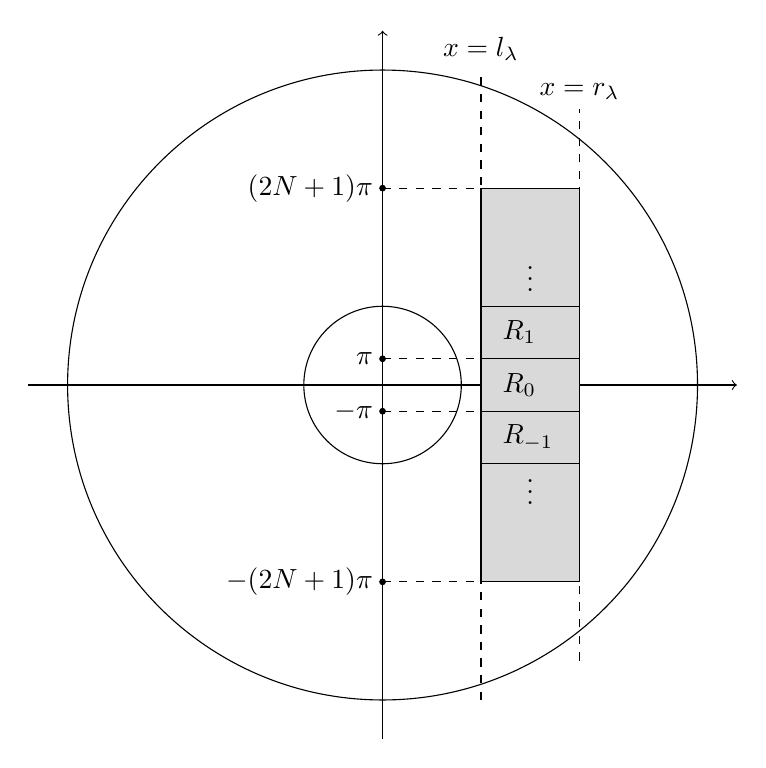
\begin{tikzpicture}
\definecolor{siva}{gray}{0.75}

\draw[->] (-4.5, 0) -- (4.5, 0);
\draw[->] (0, -4.5) -- (0, 4.5);

\draw (0, 0) circle (1);
\draw (0, 0) circle (4);

\draw[dashed] (1.25, -4) -- (1.25, 4)
node[anchor=south] {$x = l_\lambda$};
\draw[dashed] (2.5, -3.5) -- (2.5, 3.5)
node[anchor=south] {$x = r_\lambda$};

\draw[fill=gray!30] (1.25, -2.5) rectangle (2.5, 2.5);

\draw[dashed] (0, 2.5) -- (1.25, 2.5);
\draw[dashed] (0, 0.333) -- (1.25, 0.333);
\draw[dashed] (0, -0.333) -- (1.25, -0.333);
\draw[dashed] (0, -2.5) -- (1.25, -2.5);

\draw (1.25, 2.5) -- (2.5, 2.5);
\draw (1.25, 1) -- (2.5, 1);
\draw (1.25, 0.333) -- (2.5, 0.333);
% \draw[dashed] (1.25, 0) -- (2.5, 0);
\draw (1.25, -0.333) -- (2.5, -0.333);
\draw (1.25, -1) -- (2.5, -1);
\draw (1.25, -2.5) -- (2.5, -2.5);

\filldraw[black] (0, 2.5) circle (1pt)
    node[left]  {$(2N + 1) \pi$};
\filldraw[black] (0, 0.333) circle (1pt)
    node[left]  {$\pi$};
\filldraw[black] (0, -0.333) circle (1pt)
    node[left]  {$-\pi$};
\filldraw[black] (0, -2.5) circle (1pt)
    node[left]  {$-(2N + 1) \pi$};

% \draw[->] (4, 2) -- (2, 0.7);
% \draw[->] (4, 1) -- (2, 0.2);
% \draw[->] (4, -1) -- (2, -0.7);

\node[anchor=west] at (1.4, 0.67) {$R_1$};
\node[anchor=west] at (1.4, 0) {$R_0$};
\node[anchor=west] at (1.4, -0.67) {$R_{-1}$};
\node[anchor=center] at (1.875, -1.25) {$\vdots$};
\node[anchor=center] at (1.875, 1.45) {$\vdots$};

\end{tikzpicture}
    \caption{Ilustracija konstrukcije. Sivi pravokotnik je \(B (N)\).}
    \label{fig:konstrukcija}
\end{figure}
Preslikava \(E_\lambda\) desno stranico pravokotnika \(B (N)\) preslika v krožnico s središčem v izhodišču in polmerom \(\lambda e^{r_\lambda}\), medtem ko se leva stranica preslika v krog s središčem v izhodišču in radijem \(\lambda e^{l_\lambda}\). Oglejmo si kolobar
\[A = \{z : \lambda e^{l_\lambda} \leq |z| \leq \lambda e^{r_\lambda}\}.\]
Dokazali bomo, da ima \(A\) naslednji dve lastnosti.

\vspace{5mm}
\noindent \textbf{Lastnost 1}. Velja \(B (N) \subset \Int (A)\). Res, naj  bo \(z = x + i y \in B (N)\). Po definiciji \(B (N)\) imamo
\[l_\lambda \leq x \leq r_\lambda, \qquad - (2N + 1) \pi \leq y \leq (2N + 1) \pi.\]
Zato
\[|z| \leq |x| + |y| \leq r_\lambda + (2N + 1) \pi < \lambda e^{r_\lambda},\]
kar pomeni, da je \(|z|\) strogo manjše od zunanjega radija \(A\). Po drugi strani pa je
\[|z| \geq l_\lambda > \lambda e^{l_\lambda},\]
torej je \(|z|\) strogo večji od notranjega radija \(A\).

\noindent \textbf{Lastnost 2}. Funkcija \(E_\lambda\) preslika \(B (N)\) v \(A\). Res, naj bo \(z \in B (N)\). Potem \(E_\lambda (z) = \lambda e^x e^{i y}\) in zato
\[|E_\lambda (z)| = \lambda e^x \leq \lambda e^{r_\lambda} \qquad \text{in} \qquad |E_\lambda (z)| = \lambda e^x \geq \lambda e^{l_\lambda}.\]
\vspace{5mm}

\noindent Vrnemo se nazaj k konstrukciji. Za vsak \(i = -N, \dots, N\) definiramo `podpravokotnik'
\[R_i \coloneq \set{x + iy \in \CC : x \in [l_\lambda, r_\lambda], y \in [(2i - 1) \pi, (2i + 1) \pi]}.\]
Ker po lastnosti 2 \(E_\lambda\) preslika \(R_i\) v \(A\), ostaja pokazati le, je ta preslikava surjektivna. Naj bo \(w = r \lambda e^{i \theta} \in A\), torej \(r \in (e^{l_\lambda}, e^{r_\lambda})\) in \(\theta \in [(2i - 1) \pi, (2i + 1) \pi]\). Če vzamemo \(x = \ln r\) in postavimo \(z = x + i \theta\), je po definiciji \(z \in R_i\) in
\[E_\lambda (z) = \lambda e^x e^{i \theta} = \lambda r e^{i \theta} = w.\]
Tako je res \(E_\lambda (R_i) = A\). Ker to drži za vsak \(i = -N, \dots, N\), sledi tudi, da je za poljubna \(i, j\): \(R_j \subset E_\lambda (R_i)\).

Po točki (3) trditve \ref{prop:trinajst} obstaja \(\mu > 1\), da velja
\begin{equation} \label{eqn:mu-ocena}
    \bigl| E_\lambda' (z) \bigr| \geq \mu > 1 \qquad \text{na polravnini } \re z \geq l_\lambda.
\end{equation}
Zato je ta neenakost izpolnjena tudi na vsakem podpravokotniku \(R_i\). Definiramo
\[\Lambda_N \coloneq \set{z \in B(N) : E_\lambda^j (z) \in B (N) \text{ za vse } j \geq 0},\]
to je množico točk, katerih orbite pod \(E_\lambda\) ostanejo v \(B (N)\). Za vsak \(k = -N, \dots, N\) uvedemo trak
\[S (k) \coloneq \set{x + i y \in \CC : (2k - 1) \pi \leq y \leq (2k + 1) \pi}.\]
Naj bo \(L_k\) veja inverza preslikave \(E_\lambda\), definirana na pozitivno zarezani ravnini \(\CC \setminus [0, \infty)\) tako da
\[L_k (z) = \ln \prt{\frac{|z|}{\lambda}} + i \Arg_k (w),\]
kjer je \(\Arg_k (w) \in [(2k - 1) \pi, (2k + 1) \pi]\). Potem za vsak \(w \in \CC \setminus [0, \infty)\) in \(k = - N, \dots, N\) drži
\begin{equation} \label{eqn:inverz-e}
    E_\lambda \circ L_k (w) = w.
\end{equation}

\begin{trditev} \label{prop:claim}
    Za vsaka \(j, k \in \{-N, \dots, N\}\) velja \(L_k (R_j) \subset \Int (R_k)\).
\end{trditev}

\begin{dokaz}
    Ker je \(R_j \subset A\), lahko vsak \(w \in R_j\) izrazimo kot \(w = r \lambda e^{i \theta}\), kjer je \(r \in (e^{l_\lambda}, e^{r_\lambda})\) in \(\theta \in ((2k - 1) \pi, (2k + 1) \pi)\). Ker je veja inverza \(L_k\) podana z \(L_k (w) = \ln r + i \theta\) dobimo \(L_k (w) \in \Int (R_k)\).
\end{dokaz}

Za nek \(z \in \Lambda_N\) je \(\im (E_\lambda^n (z)) \neq (2j \pm 1) \pi\) za vsak \(n \in \NN\) in vsak \(j = -N, \dots, N\). Res, če je \(E_\lambda^n (z) = x + (2j \pm 1) \pi i\), potem je \(E_\lambda^{n + 1} (z) = - \lambda e^x \notin B (N)\). Zato vsaka točka \(E_\lambda^n (z)\) leži v pravokotniku
\[R_i^* \coloneq \set{x + iy \in \CC : x \in [l_\lambda, r_\lambda], y \in ((2i - 1) \pi, (2i + 1) \pi)},\]
ki ga dobimo, če pravokotniku \(R_i\) odstranimo zgornjo in spodnjo stranico. Tako vsak \(z \in \Lambda_N\) določa svoje natanko določeno zaporedje
\[\overline{s} = (s_0, s_1, s_2, \dots), \qquad s_i \in \{-N, \dots, N\}\]
za katerega velja
\begin{equation} \label{eqn:itinerar}
    E_\lambda^n (z) \in R_{s_n}^* \qquad \text{za vsak } n = 0, 1, \dots
\end{equation}
Zaporedje \(\overline{s}\) imenujemo \emph{itinerar} točke \(z\). Ker je po definiciji veje \(L_{s_n}\) za vsak \(w = E_\lambda^n (z) \in R_{s_n}^*\) prav tako \(L_{s_n} (E_\lambda (w)) = w\) sledi
\begin{equation} \label{eqn:devetpet}
    L_{s_n} \circ E_\lambda \prt{E_\lambda^n (z)} = E_\lambda^n (z).
\end{equation}

V nadaljevanju pokažemo, da za vsak \(\overline{s} \in \Sigma_N\) množica
\[\bigcap_{n \geq 0} L_{s_0} \circ \dots \circ L_{s_{n - 1}} \prt{B (N)} \coloneq \bigcap_{n \geq 1} L_s^{[n]} \prt{B (N)}\]
vsebuje natanko eno točko, ki jo označimo z \(z_{\overline{s}}\). Ker je po trditvi \ref{prop:claim} za vsak \(j, k\)
\[L_k (R_j) \subset \Int (R_k) \implies L_s^{[n + 1]} \prt{B (N)} \subset L_s^{[n]} \prt{B (N)},\]
je zaporedje množic \(\{L_s^{[n]} (B (N))\}_{n = 1}^{\infty}\) padajoče. Da je njihovo presečišče zgolj ena točka, zadostuje, da zaporedje njihovih premerov
\[d_n \coloneq \diam \prt{L_s^{[n]} \prt{B (N)}}\]
konvergira proti \num{0}. Naj bosta \(z_1, z_2 \in B(N)\). Z neenakostjo \(|E_\lambda' (z)| \geq \mu > 1\) (enačba \eqref{eqn:mu-ocena}) in enakostjo \eqref{eqn:devetpet} ter verižnim pravilom dobimo
\[\prt{L_s^{[n]}}' (z) = \prt{E_\lambda^n}' \prt{L_s^{[n]} (z)}^{-1} \implies \abs{\prt{L_s^{[n]}}' (z)} \leq \mu^{- (n + 1)}.\]
Zato
\[ \begin{multlined}[12cm]
    \left| L_s^{[n]}(z_2) - L_s^{[n]}(z_1) \right| = \left| \int_{z_1}^{z_2} \prt{L_s^{[n]}}' (z) \, \dd z \right|\\
    \leq |z_2 - z_1| \cdot \sup_{z \in B(N)}\left| \left( L_s^{[n]} \right)'(z) \right| \leq \frac{\diam (B(N))}{\mu^{n+1}}.
\end{multlined} \]
Ker je \(\mu > 1\), desna stran konvergira proti \num{0} in zato tudi \(d_n\) konvergirajo proti \num{0}.

\begin{izrek}
    Preslikava \(\phi \colon \Sigma_N \to \Lambda_N\); \(\phi (\overline{s}) = z_{\overline{s}}\) je homeomorfizem, ki konjugira skrčitev \(E_\lambda\) na \(\Lambda_N\) ter preslikavo zamika \(\sigma\). 
\end{izrek}

\begin{dokaz}
    (1) \textbf{Surjektivnost}. Naj bo \(\overline{s} \in \Sigma_N\) itinerar točke \(z \in \Lambda_N\). Z indukcijo pokažemo, da je \(\phi (\overline{s}) = z\). Za \(n = 0\) po definiciji \(z \in B (N)\) velja \(L_{s_0} \circ E_\lambda (z) = z\). Predpostavimo
    \[z = L_{s}^{[n]} \prt{E_{\lambda}^{n + 1} (z)}.\]
    Potem iz enačbe \eqref{eqn:devetpet} in verižnega pravila sledi
    \[L_{s}^{[n + 1]} \prt{E_{\lambda}^{n + 2} (z)} = L_{s}^{[n]} \prt{L_{s_{n + 1}} \circ E_\lambda (E_\lambda^{n + 1} (z))} = L_{s}^{[n]} \prt{E_\lambda^{n + 1} (z)} = z.\]
    S tem smo pokazali, da je \(z \in L_{s_0} \circ L_{s_1} \circ \dots \circ L_{s_n} (B (N))\) za vsak \(n \geq 0\) in zato \(z = \phi (\overline{s})\).

    (2) \textbf{Surjektivnost}. Naj bosta \(\overline{s}, \overline{s}^* \in \Sigma_N\), da \(\overline{s} \neq \overline{s}^*\). Naj bo \(j \in \NN\) najmanjši, da je \(s_j \neq s_j^*\). Če bi veljalo \(\phi (\overline{s}) = \phi (\overline{s}^*) = z\), bi po definiciji itinerarja veljalo
    \[E_\lambda^j (z)\in L_{s_j} \prt{B (N)} \cap L_{s_j^*} \prt{B (N)}.\]
    A za \(w \in L_{s_j} \prt{B (N)}\) je imaginarni del \(\im w \in ((2 s_j - 1) \pi, (2 s_j + 1) \pi)\), za \(w^* \in L_{s_j^*} \prt{B (N)}\) pa \(\im w^* \in ((2 s_j^* - 1) \pi, (2 s_j^* + 1) \pi)\). Ker sta ta intervala disjunktna, je to protislovje.

    (3) \textbf{Zveznost}. Naj bo \(\overline{s}^o \in \Sigma_N\) in \(z_0 = \phi (\overline{s}^o)\). Za \(\varepsilon > 0\) izberemo tak \(k\), da
    \[\frac{\diam (B (N))}{\mu^{k + 1}} < \varepsilon,\]
    kjer je \(\mu > 1\) iz ocene \(|E_\lambda'| \geq \mu\) \eqref{eqn:mu-ocena}. Potem ima vsak \(\overline{s}\) iz okolice
    \[U = \set{\overline{s} \in \Sigma_N : s_i = s_i^o \text{ za } 0 \leq i \leq k}\]
    prvih \((k + 1)\) simbolov enakih kot \(\overline{s}^o\). Tako za obe točki \(\phi (\overline{s})\) in \(\phi (\overline{s}^o)\) velja
    \[\phi (\overline{s}), \phi (\overline{s}^o) \in L_s^{[k + 1]} \prt{B (N)}.\]
    Iz neenakosti v dokazu konvergence premerov \(d_n\) tudi tukaj sledi
    \[\left| \phi (\overline{s}) - \phi (\overline{s}^o) \right| \leq \diam \prt{B (N)} \frac{1}{\mu^{k + 1}} < \varepsilon.\]
    Tako je \(\phi\) zvezna.

    (4) \textbf{Zveznost inverza}. Ker je \(\Sigma_N\) kompakten in \(\phi\) bijektivna, je \(\phi^{-1}\) zvezna.

    (5) \textbf{Konjugacija}. Če je \((s_0, s_1, s_2, \dots) = \phi^{-1} (z)\), potem je \(z \in L_s^{[n]} \prt{B (N)}\) za vsak \(n \in \NN\) in zato \(E_\lambda (z) \in E_\lambda \circ L_s^{[n]} \prt{B (N)}\) za vsak \(n \in \NN\). Uporabimo \eqref{eqn:inverz-e}, da dobimo \(E_\lambda (z) \in L_s^{[n]} \prt{B (N)}\) za vsak \(n \in \NN\). To pomeni \(E_\lambda (z) = \phi (s_1, s_2, \dots) = \phi \circ \sigma (s_0, s_1, s_2, \dots) = \phi \circ \sigma \circ \phi^{-1} (z)\).
\end{dokaz}

\noindent Končno lahko dokažemo enakost
\[\overline{\bigcup_{n \geq 1} \Lambda_N} = J (E_\lambda).\]
Po neenakosti \(|E_\lambda' (z)| \geq \mu > 1\) \eqref{eqn:mu-ocena} za vsak \(z \in \Lambda_N\) in izreku \ref{thm:julm} je \(\Lambda_N \subset J (E_\lambda)\). Ker je \(J (E_\lambda)\) zaprtje množice vseh odbojnih periodičnih točk je dovolj, da dokažemo, da je vaka taka točka v kakšni od množic \(\Lambda_N\). Naj bo \(z_0\) odbojna periodična točka preslikave \(E_\lambda\). S posledico \ref{cor:jul-e} vemo, da \(z \in \{\re z \geq l_\lambda\}\). Periodičen cikel \(\{z_0, E_\lambda (z_0), \dots\}\) je tako omeje na polravnini \(\{\re z \geq l_\lambda\}\), zato je za dovolj velik \(N\) v celoti vsebovan v \(B (N)\). Po definiciji \(\Lambda_N\) so vse točke cikla v \(\Lambda_N\), torej je tudi \(z_0 \in \Lambda_N\).

